% !TEX program = xelatex
\documentclass[12pt]{article}
\usepackage[margin=1in]{geometry}
\usepackage{nopageno} % no page numbers
\usepackage{setspace} \doublespacing

\usepackage{graphicx}
\graphicspath{ {./graphics/} }
\usepackage[dvipsnames]{xcolor}
\definecolor{CrispBlue}{HTML}{0176AE}

\usepackage{fontspec}
\usepackage{tcolorbox}
\usepackage{etoolbox}
\BeforeBeginEnvironment{verbatim*}{\begin{tcolorbox}[colback=CrispBlue!5!white,colframe=CrispBlue!75!black]}%
\AfterEndEnvironment{verbatim*}{\end{tcolorbox}}%

\usepackage{hyperref}
\hypersetup{
    colorlinks,
    citecolor=black,
    filecolor=black,
    linkcolor=black,
    urlcolor=black
}

\renewcommand{\footnotesize}{\fontsize{8pt}{10pt}\selectfont}


\usepackage[labelfont={small,sc,bf},textfont={small,sc,bf}]{caption}
\setlength{\parindent}{24pt}
% \setlength{\parskip}{1em}

\usepackage{tocloft}
\renewcommand{\cftpartleader}{\cftdotfill{\cftdotsep}}
\renewcommand{\cftsecleader}{\cftdotfill{\cftdotsep}}

\usepackage[shortlabels]{enumitem}

\usepackage{lastpage}
\usepackage{fancyhdr}
\pagestyle{fancy}
\fancyhf{}
\renewcommand{\headrulewidth}{0pt}
\rfoot{Page \thepage\ of \pageref*{LastPage}}

\usepackage{amsmath,amsfonts,amssymb}
\usepackage{bm}
\usepackage{mathtools}

\renewcommand{\listfigurename}{List of Figures}

\begin{document}
\setmainfont{SF Pro Text}
\setsansfont{SF Pro Text}
\setmonofont{SF Mono}
\renewcommand{\familydefault}{\sfdefault}

\hypersetup{
    linkcolor=CrispBlue,
    urlcolor=CrispBlue,
    breaklinks=true
}

\noindent David Kirby\\
ECE 529: Introduction to Technical Cybersecurity\\
Spring, 2022
\begin{center}
    \large\bfseries Detailed Scan Report
\end{center}

This assignment, part of the Reconnaissance and Vulnerability Identification\footnote{\href{https://learn.unm.edu/webapps/assignment/uploadAssignment?content_id=_7770481_1&course_id=_110809_1&user_id=_196414_1}{https://learn.unm.edu/webapps/assignment/uploadAssignment?content\_id=\_7770481\_1\&course\_id=\_110809\_1}} module, was designed to introduce students to the nmap scanning tool and to produce a detailed scan report for different hosts. The first host to be scanned was Metasploitable\footnote{\href{https://www.metasploit.com}{https://www.metasploit.com}} from Rapid7 -- a virtual machine that is built from the ground up with a large amount of security vulnerabilities. Metasploitable is intended purely for testing and pedagogical purposes as these vulnerabilities make it similar to many embedded Linux IoT devices. The other host to be scanned was an LTS (long term support) version of Ubuntu\footnote{\href{https://ubuntu.com/blog/what-is-an-ubuntu-lts-release}{https://ubuntu.com/blog/what-is-an-ubuntu-lts-release}}, which one assumes is stable and free of many vulnerabilities. To perform our penetration testing we used Kali Linux\footnote{\href{https://www.kali.org}{https://www.kali.org}}, a distribution specifically optimized with tools for security professionals. This module presented a particular challenge as I am using an M1 Mac, and while there are ARM distributions for Kali Linux and Ubuntu Server, there is not a suitable ARM distribution for Metasploitable. This made connecting the distributions to the same subnet a novel challenge. I will quickly run through the attempts that failed before presenting the final solution.

\begin{figure}[!ht]
    \centering
    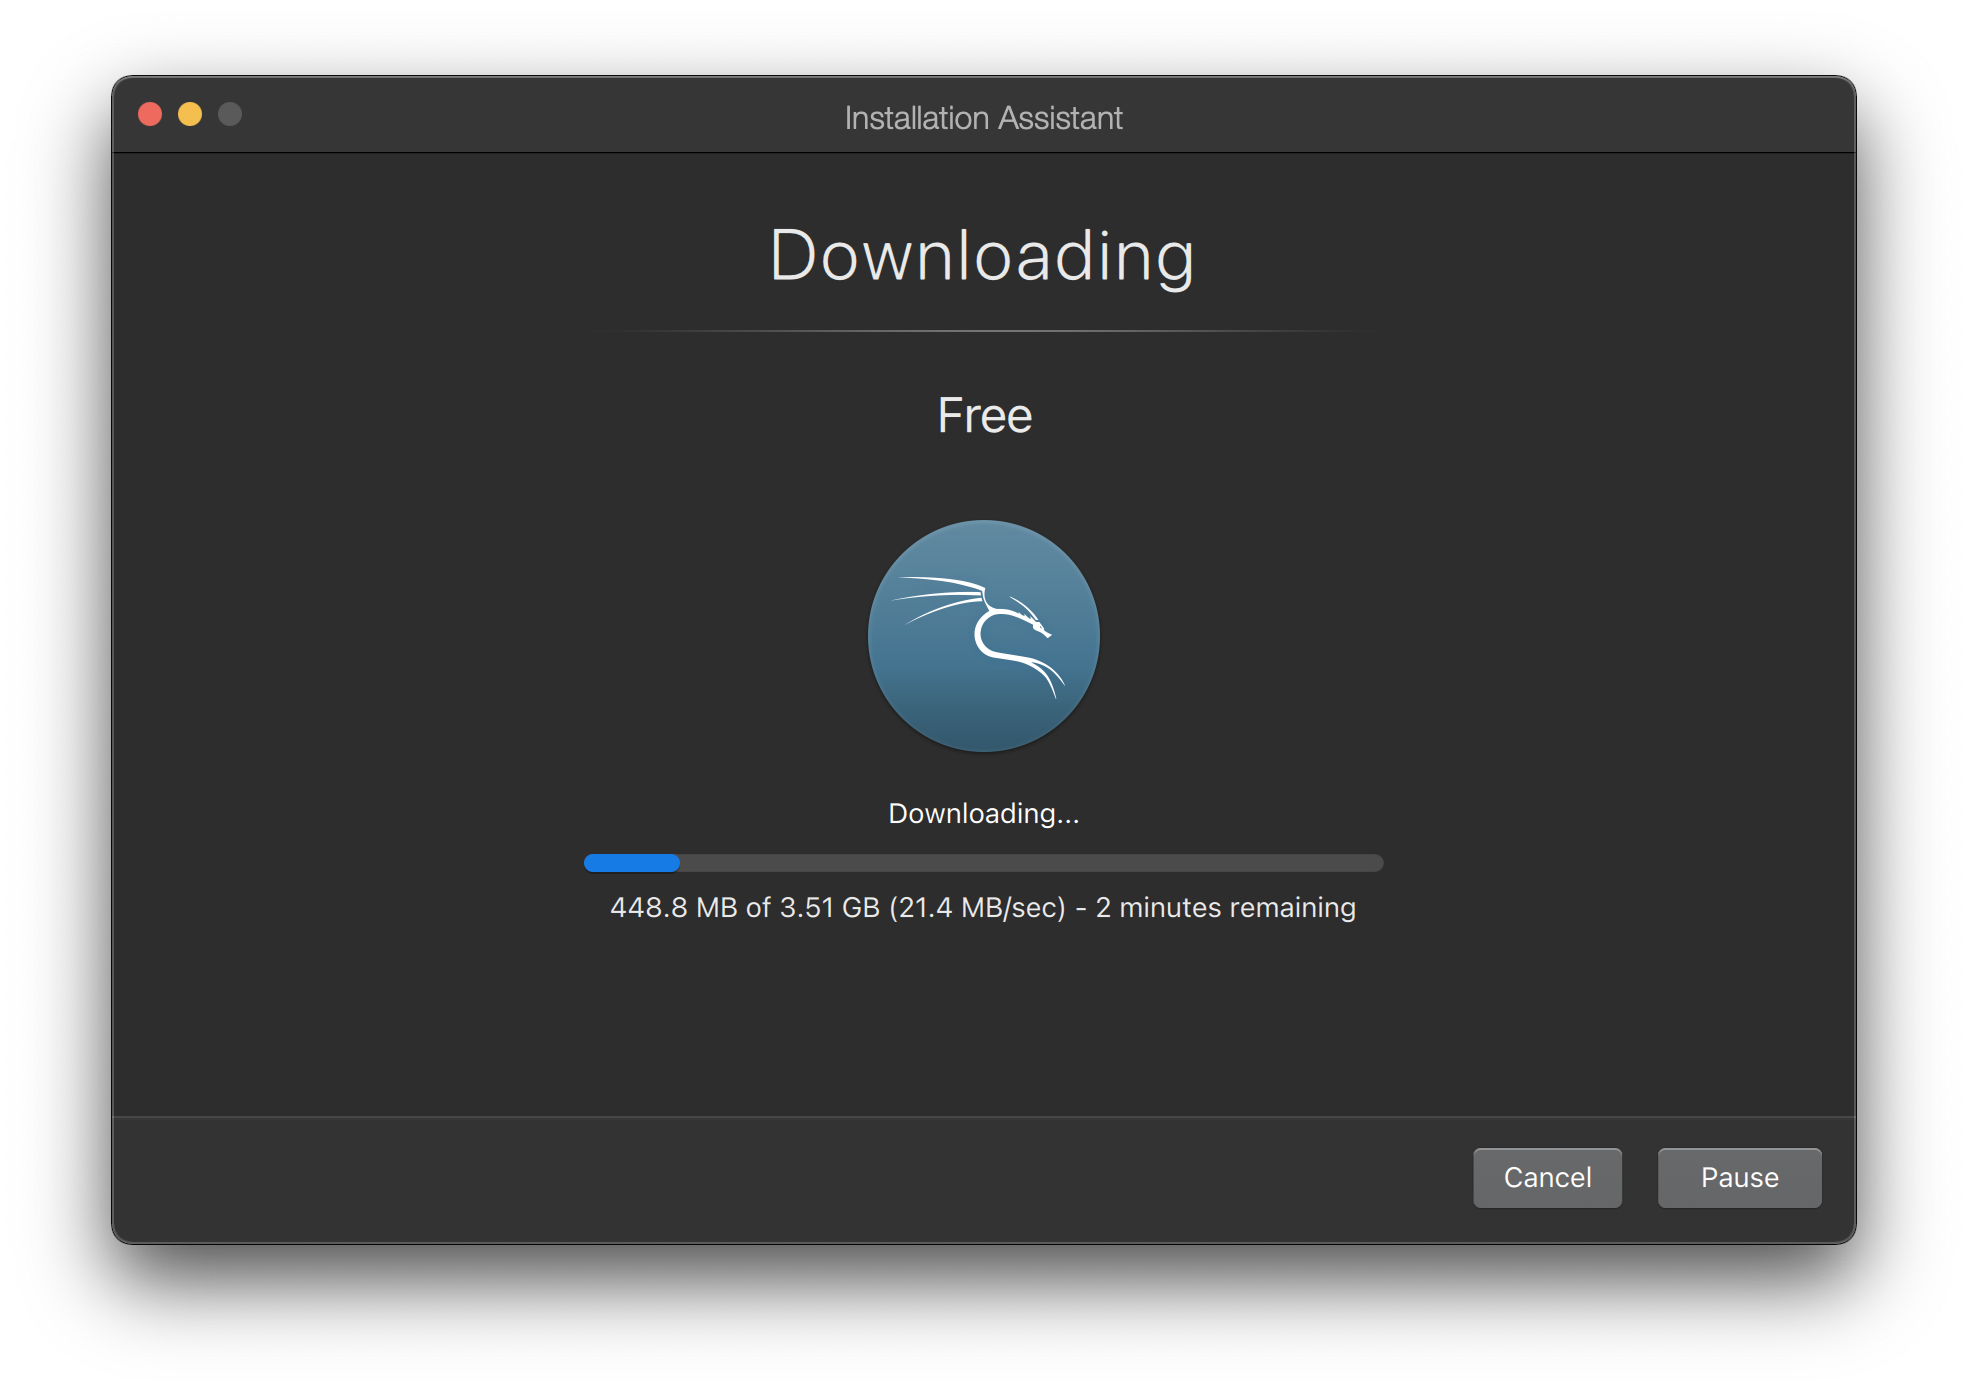
\includegraphics[width=0.9\textwidth]{figure01.png}\vspace{-1em}
    \caption{Kali Linux Installation Using Parallels Desktop.}
    \label{fig:Kali}
\end{figure}

Having taken a cloud computing course in a previous semester, I had a suitable VM of Ubuntu Server (20.04.3 LTS) updated and ready to deploy. As my virtualization software, I used Parallels Desktop which runs natively on Apple silicon. With one host solved, the next step was to install Kali Linux. This was a simple enough process as Parallels offered a one-step install (see Figure~\ref{fig:Kali}). This installation allowed me to configure two different networks as called for in the assignment -- a bridge network connected to the Mac's outward facing network, and a host network designed to set up a private subnet for the three VMs. I was able to ping the host machine (macOS), the Ubuntu VM, as well as the outside world; however, the next step would prove to be the wrench in the machine. When trying to install Metasploitable, Parallels kicked back an error stating that x86 VMs were not able to be run on Apple silicon (at this time). Macs with Apple silicon implement Rosetta 2 which literally translate\footnote{\href{https://support.apple.com/en-us/HT211861}{https://support.apple.com/en-us/HT211861}} the CISC instruction set to RISC on initial run, and then subsequently run the translated code. This is what makes Rosetta 2 so efficient, to the point where some code runs faster emulated on M1 than natively\footnote{\href{https://www.macrumors.com/2020/11/15/m1-chip-emulating-x86-benchmark/}{https://www.macrumors.com/2020/11/15/m1-chip-emulating-x86-benchmark/}}. Unfortunately, VMs cannot be translated on the fly, and meant I needed to find another solution for the Metasploitable VM. My next thought was to use my wife's Intel-based Mac and create a subnet using her computer; however, knowing how vulnerable Metasploitable was, I was reluctant to expose her system. Pivoting to the next possible solution meant trying Metasploitable with a Docker container.

Docker for M1 Macs now runs natively\footnote{\href{https://www.docker.com/press-release/Docker-Desktop-for-M1-powered-Macs}{https://www.docker.com/press-release/Docker-Desktop-for-M1-powered-Macs}} and has the added bonus of being able to run x86 and amd64 distributions. As luck would have it, I was not the first to attempt to containerize Metasploitable and there were many distributions available on Docker Hub. I found a suitable one that already had the vulnerabilities opened up and set out connecting it to my ECE529 subnet. Then came another bump in the road, Docker containers are inherently isolated from their hosts. This meant I could ping my Mac, Kali, and Ubuntu VMs from Metasploitable, but none of them could ping the container -- it was isolated from the outside. There were workarounds for the Mac, but nothing that would work with Kali and Ubuntu; I was back to square one. Doing some reconnaissance, I discovered that it is possible to create custom networks within Docker and connect all of the VMs to the same subnet. The solution was not to run VMs alongside containers, but to instead run everything from within Docker. This is where past experience with containers came in handy.

\begin{figure}[!ht]
    \centering
    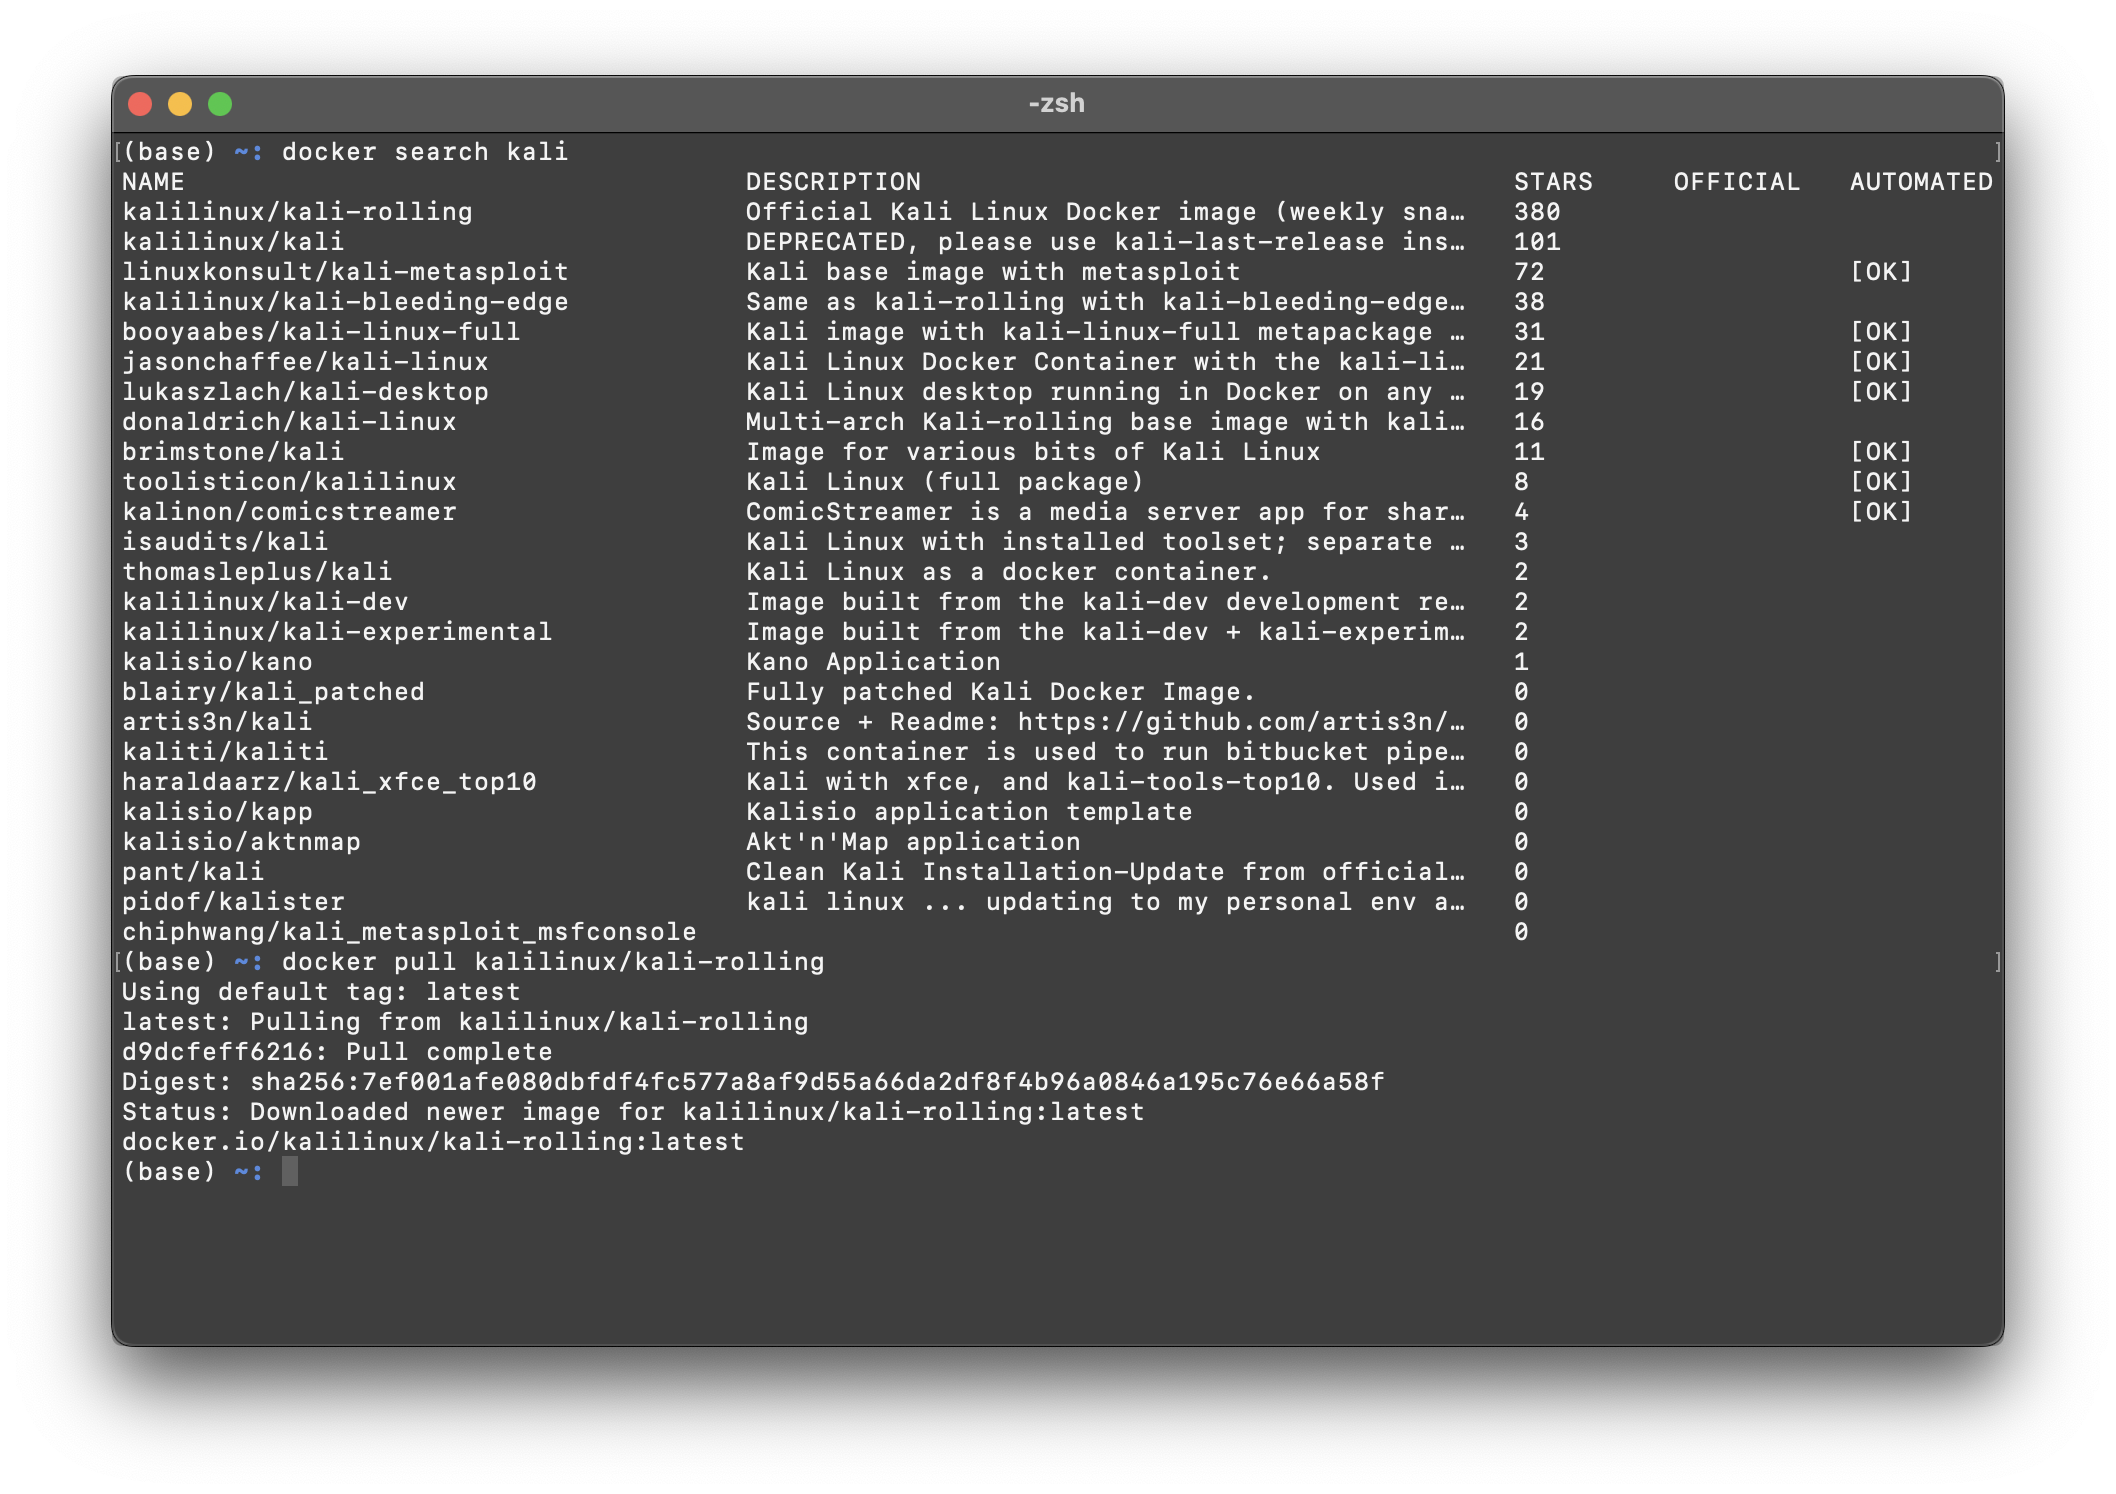
\includegraphics[width=0.8\textwidth]{figure02.png}\vspace{-1em}
    \caption{Docker Search Results for Kali Linux.}
    \label{fig:DockerSearch}
\end{figure}

\begin{figure}[!ht]
    \centering
    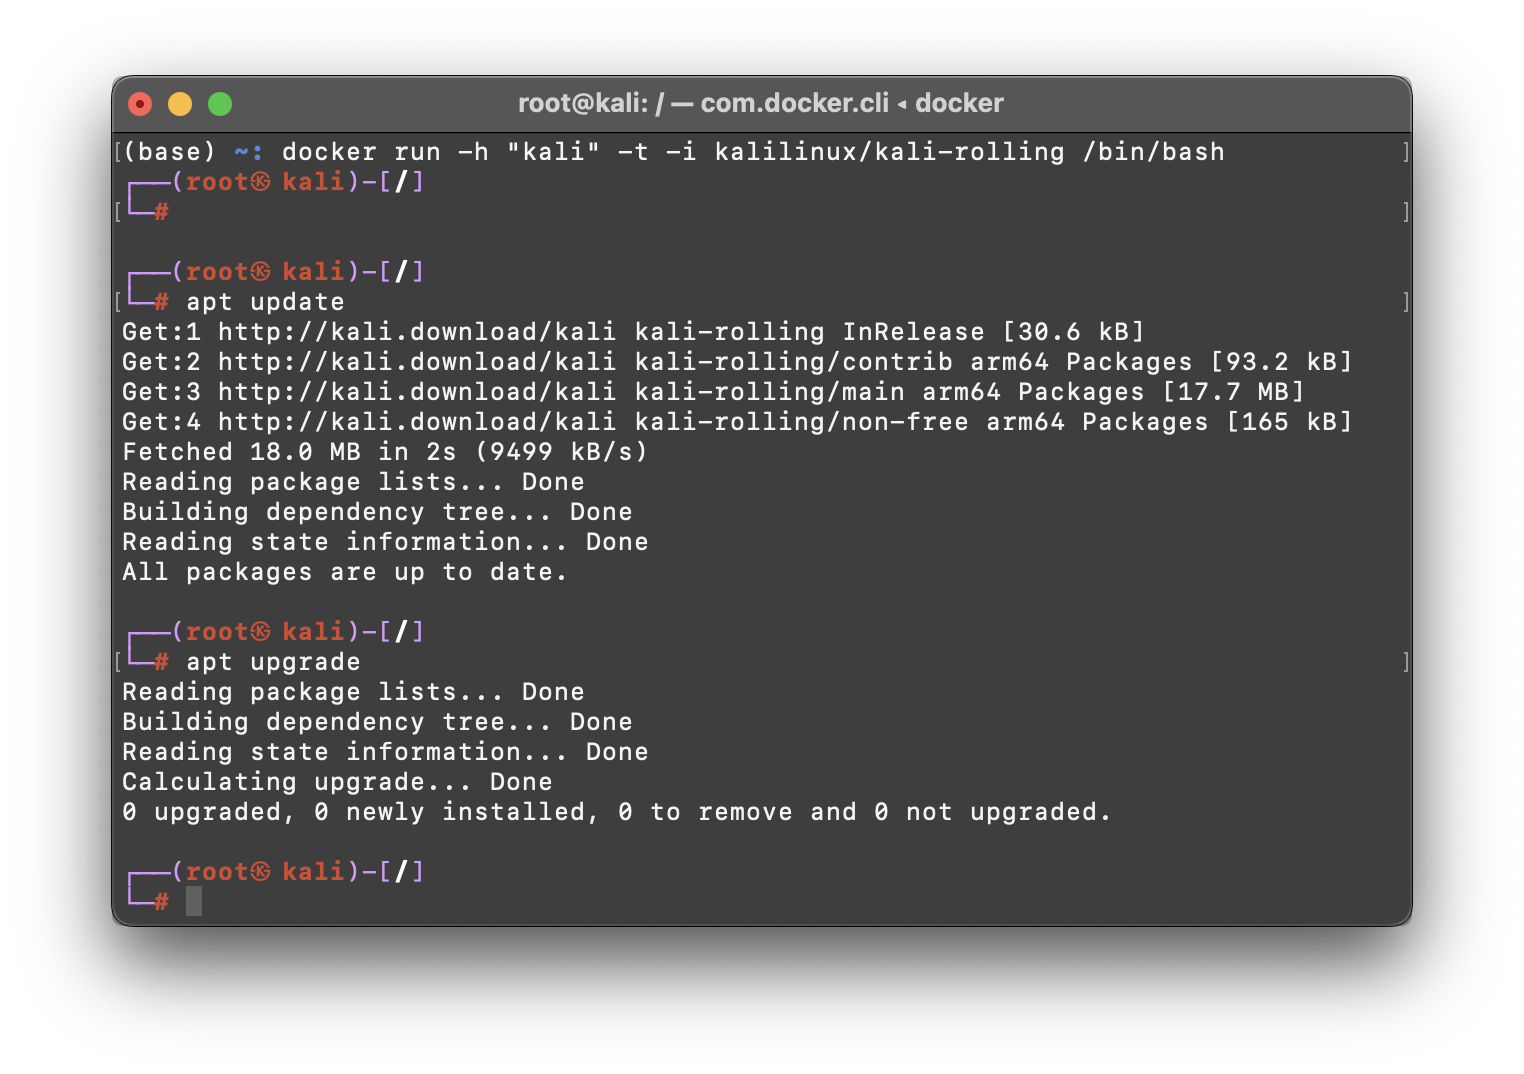
\includegraphics[width=0.7\textwidth]{figure03.png}\vspace{-1em}
    \caption{Setup Kali Linux Container.}
    \label{fig:RunKali}
\end{figure}

Searching Docker Hub for Kali Linux provided numerous results, so I chose the base, weekly-updated official image (see Figure~\ref{fig:DockerSearch}). Running the image was done so that our hostname was ``kali'' and with a bash shell as shown in Figure~\ref{fig:RunKali}. Updating did not do much, of course, as this was the latest release; however, this base system did not come with any tools. Those were easy enough to download using the Kali Linux Metapackages\footnote{\href{https://www.kali.org/docs/general-use/metapackages/}{https://www.kali.org/docs/general-use/metapackages/}} (I chose to download every tool with \texttt{kali-linux-everything}). Note: this took an incredibly long time, even over fiber optic connection, so while the container setup took less than a minute, to get Kali to a working copy took quite a bit longer. In the future, I would recommend downloading specific tools as needed. Once Kali was setup, I did the same with Ubuntu and Metasploitable, again using a container from Docker Hub that already had the vulnerabilities exposed. Finally, with all of my containers set up and connected to the same Docker-created subnet, I was able to begin testing with nmap.

\begin{figure}[!ht]
    \centering
    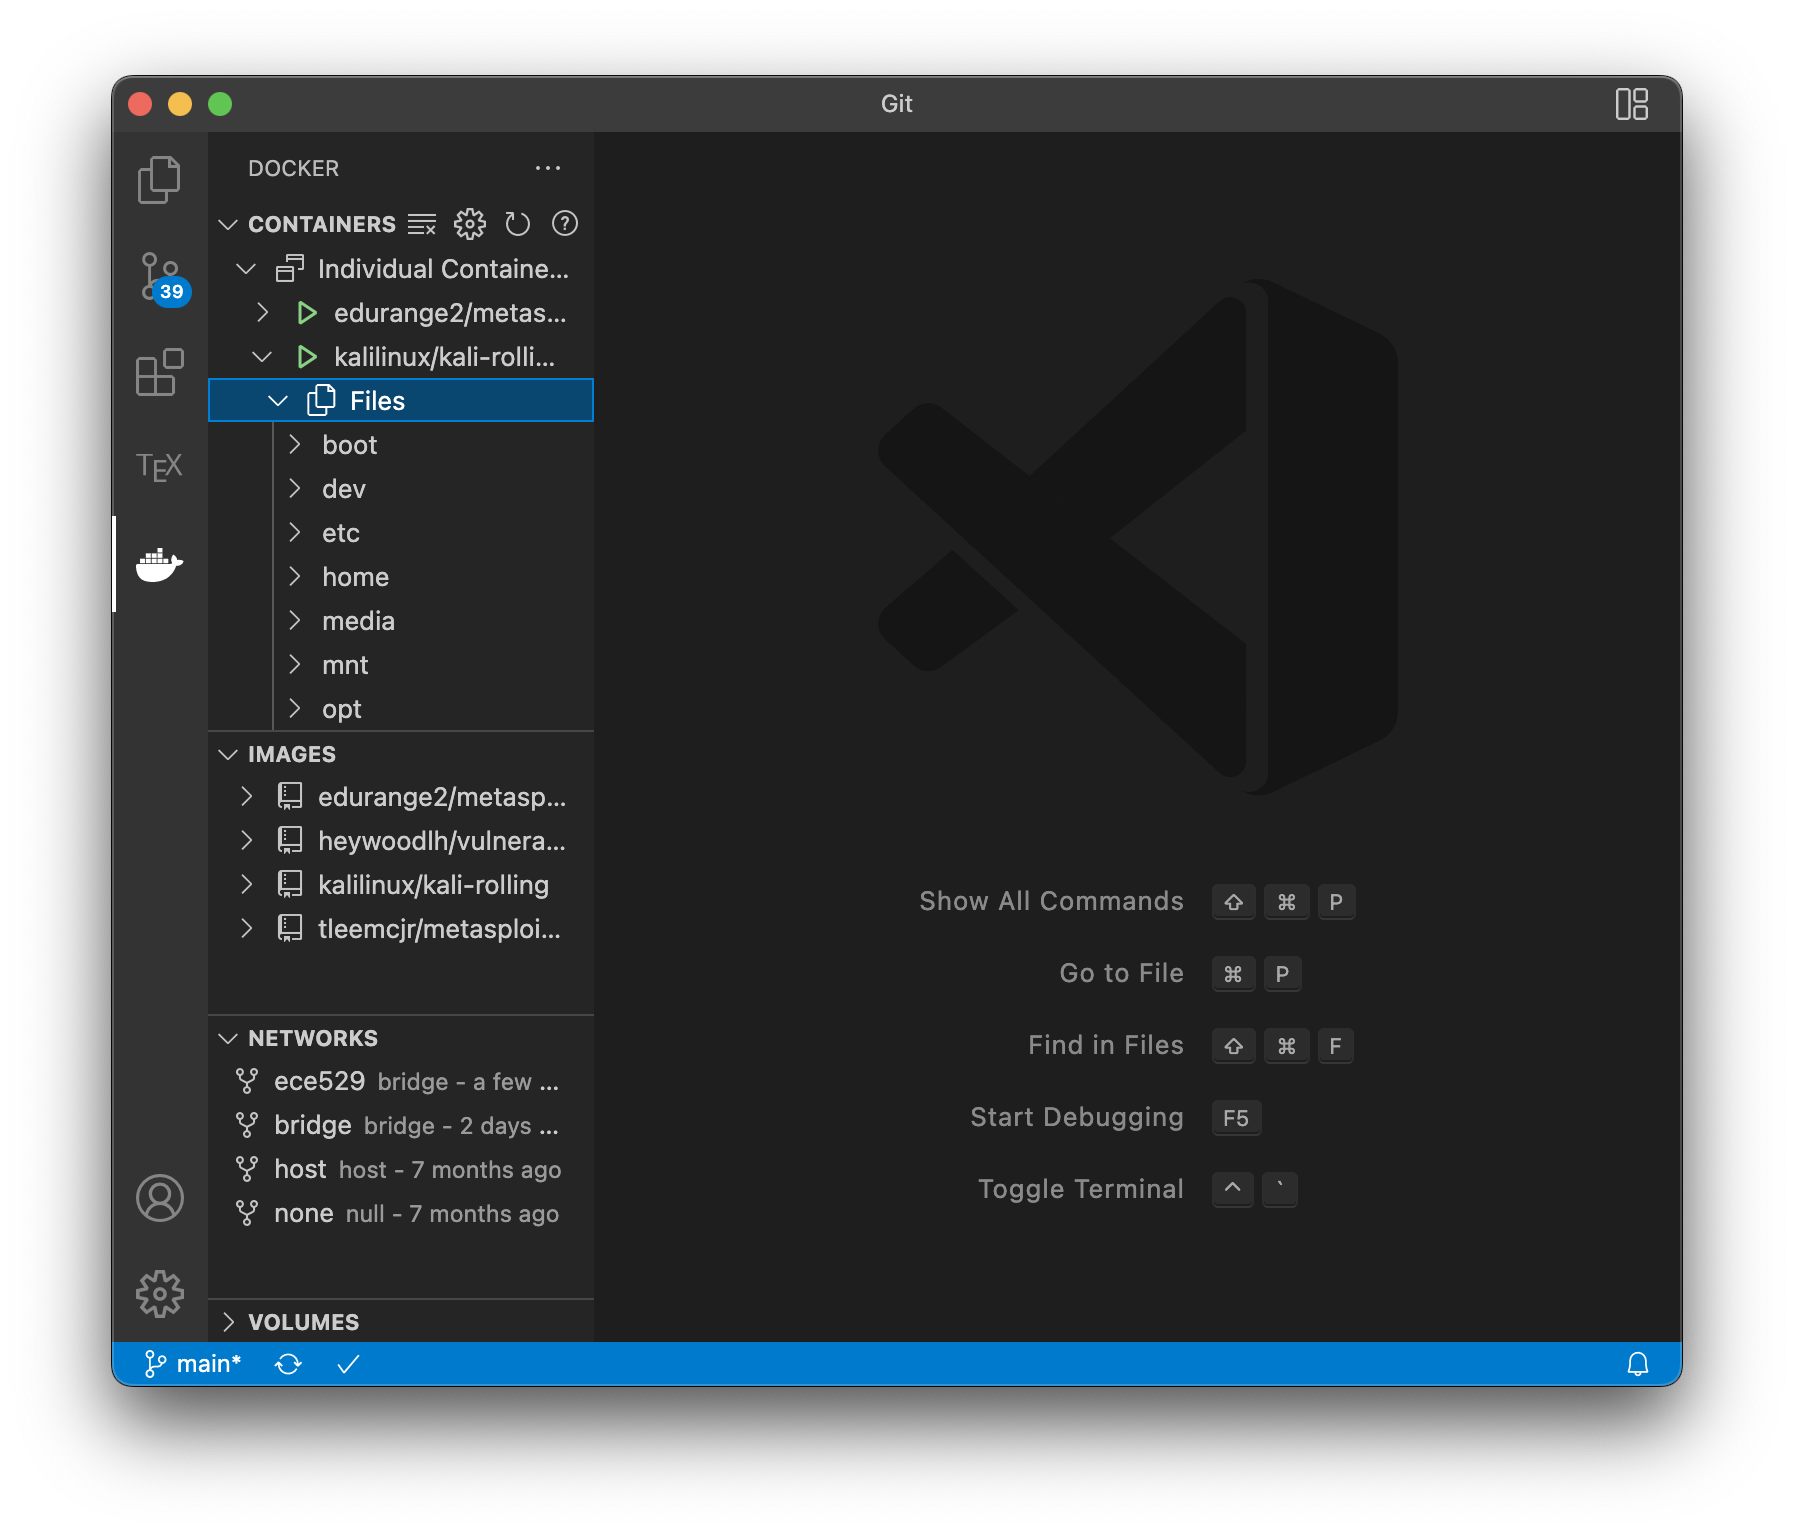
\includegraphics[width=0.8\textwidth]{figure04.png}\vspace{-1em}
    \caption{Visual Studio Code with Docker Support.}
    \label{fig:VSCode}
\end{figure}

The first submodule of Module 3 was to test nmap on our subnet and output the results to a text file and capture the packets using tcpdump to be analyzed later in Wireshark. This is typical practice and, as mentioned in the professor's videos, it is easier to capture data now for analysis later than to analyze on the fly. To obtain the files from the containers, I used Visual Studio Code and the Docker extension which lets us inspect running containers and extract files (see Figure~\ref{fig:VSCode}). This tool also allowed for us to see and configure the images and available networks. This could have been done using the command line (\texttt{docker network ls}), but having a GUI to drag and drop files and confirm networks made the process infinitely easier. The output of the text file out.txt is shown below:

\begin{tcolorbox}[colback=CrispBlue!5!white,colframe=CrispBlue!75!black,title=Output of \texttt{nmap -oN out.txt -sP 172.17.0.*}]\setstretch{1.25}\footnotesize
\begin{verbatim}
# Nmap 7.92 scan initiated Fri Feb  4 05:23:31 2022 as: nmap -oN out.txt -sP 172.17.0.*
Nmap scan report for 172.17.0.1
Host is up (0.000069s latency).
MAC Address: 02:42:98:88:21:C2 (Unknown)
Nmap scan report for 172.17.0.2
Host is up (0.000079s latency).
MAC Address: 02:42:AC:11:00:02 (Unknown)
Nmap scan report for kali (172.17.0.3)
Host is up.
# Nmap done at Fri Feb  4 05:23:33 2022 -- 256 IP addresses (3 hosts up) scanned in 1.99
 seconds
\end{verbatim}
\end{tcolorbox}

Figures~\ref{fig:nmap01} and~\ref{fig:nmap02} show the command line outputs from both our nmap terminal and tcpdump terminal, both were run simultaneously and show the containers connected to the subnet.

\begin{figure}[!ht]
    \centering
    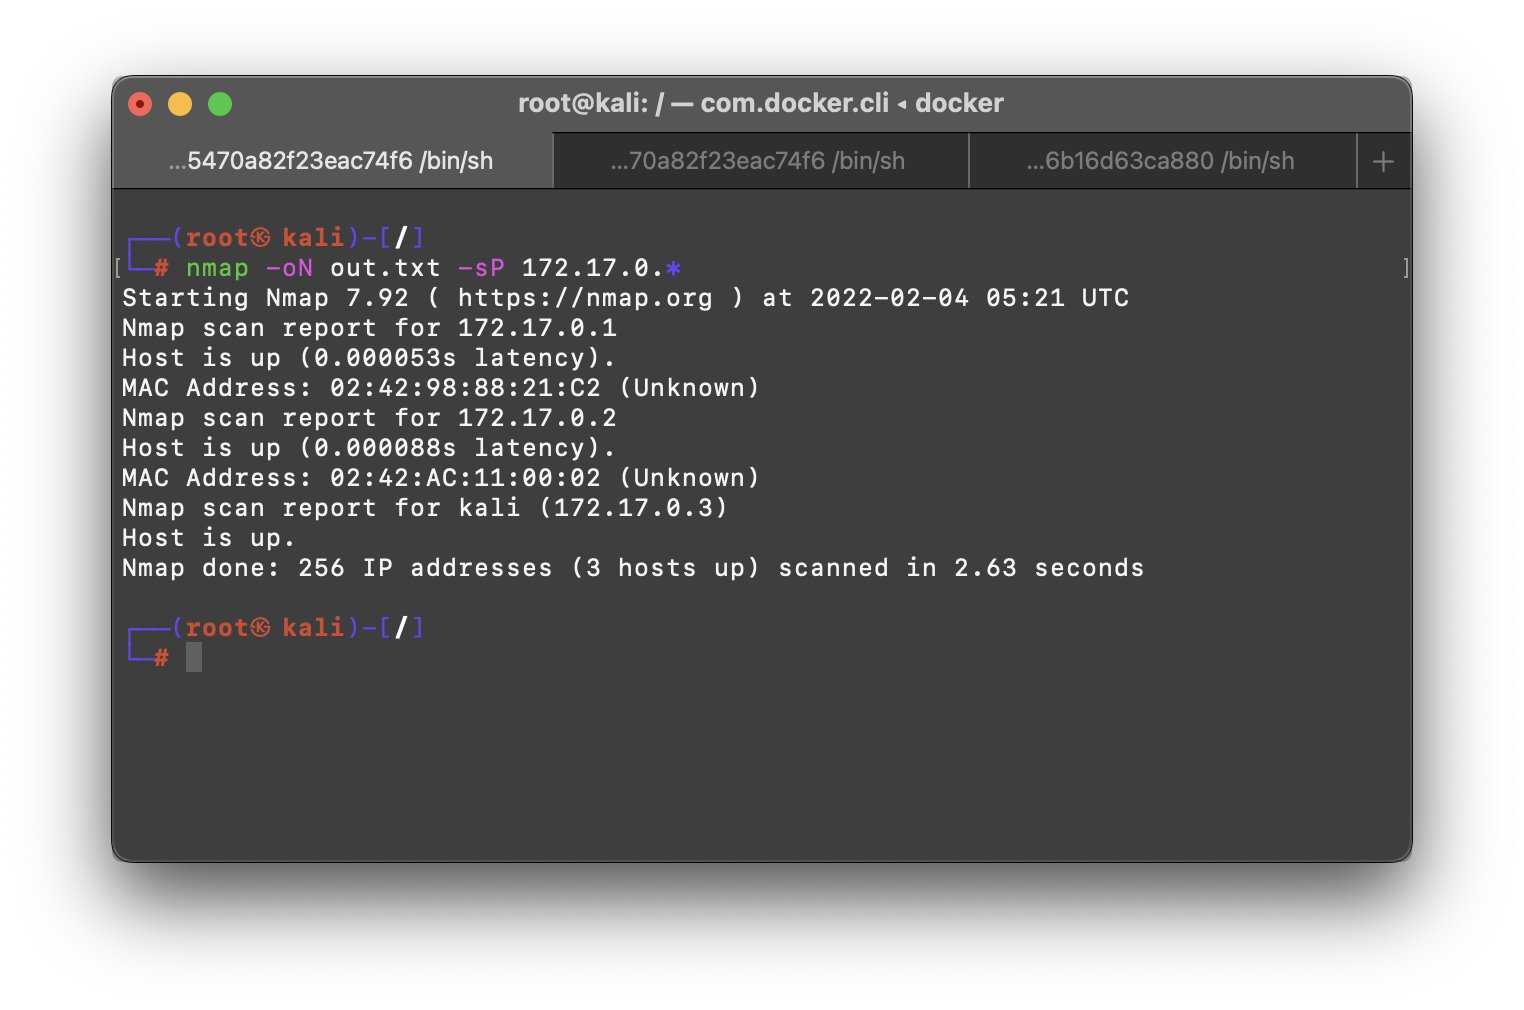
\includegraphics[width=0.7\textwidth]{figure05.png}\vspace{-1em}
    \caption{Command line for \texttt{nmap -oN out.txt -sP 172.17.0.*}.}
    \label{fig:nmap01}
\end{figure}

The second submodule involved using nmap to scan a website designed explicitly to test nmap -- scanme.nmap.org. The results in Figures~\ref{fig:nmap03} and~\ref{fig:nmap04} show that the host was up and we were able to capture ICMP echo requests and ACK packets. Further penetration tests using nmap will show ports and software running on this host. For brevity, I will omit the command line screenshots for subsequent runs and only show the text output (which is identical to the command line output).

\begin{figure}[!ht]
    \centering
    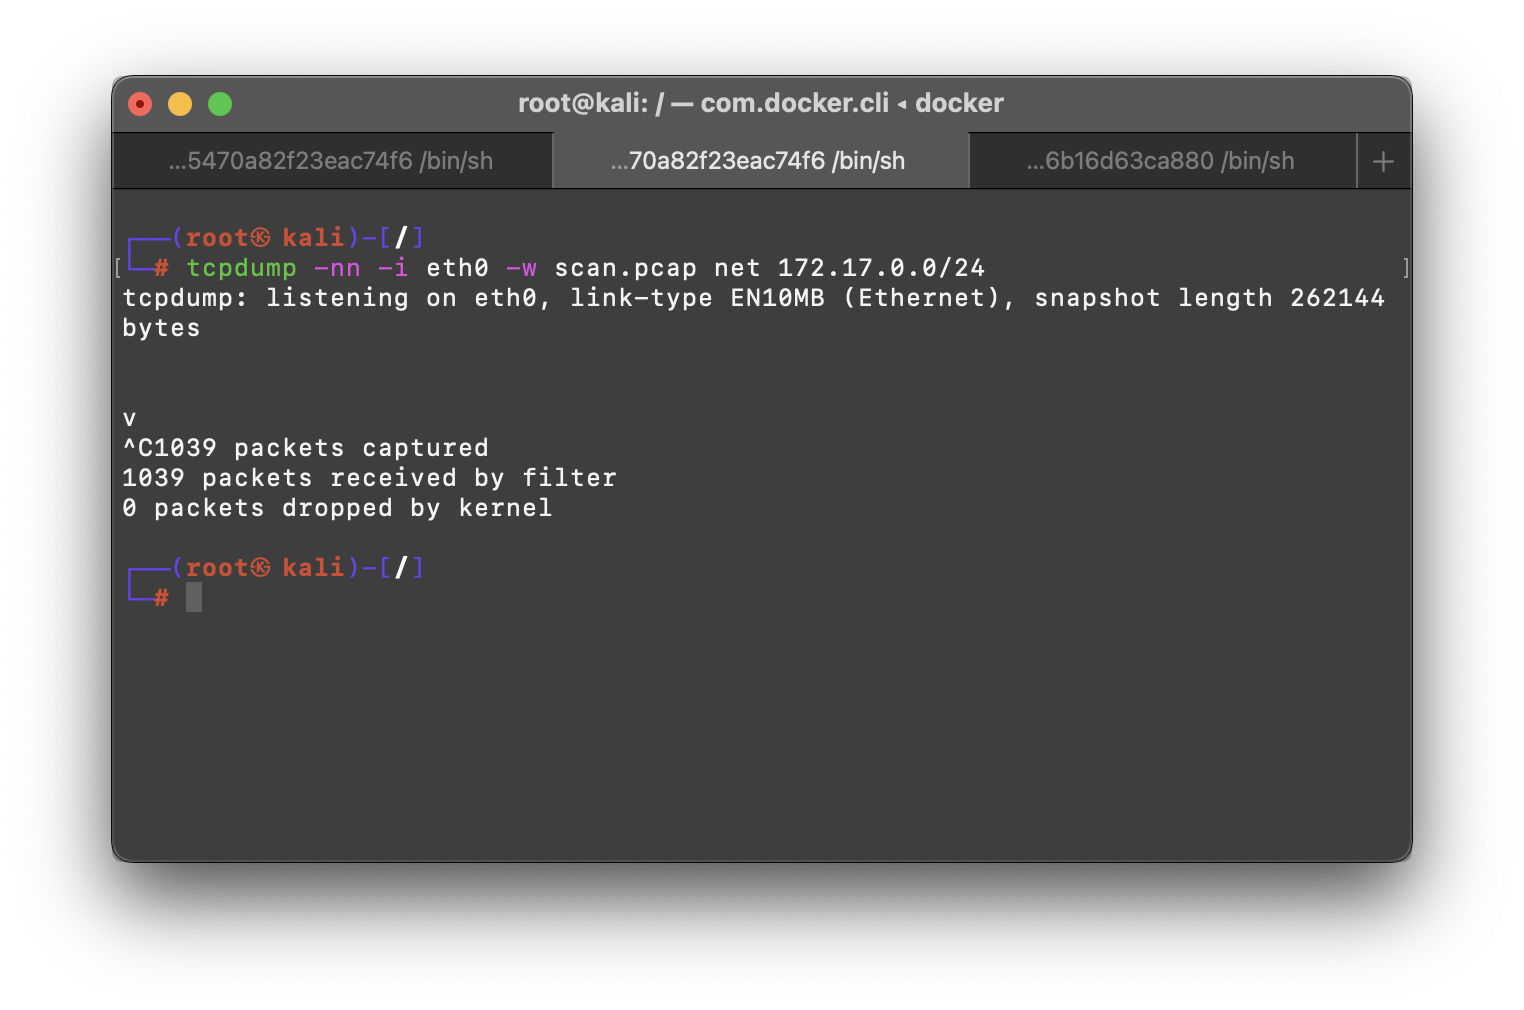
\includegraphics[width=0.6\textwidth]{figure06.png}\vspace{-1em}
    \caption{Command line for \texttt{tcpdump -nn -i eth0 -w scan.pcap net 172.17.0.0/24}.}
    \label{fig:nmap02}
\end{figure}

\begin{figure}[!ht]
    \centering
    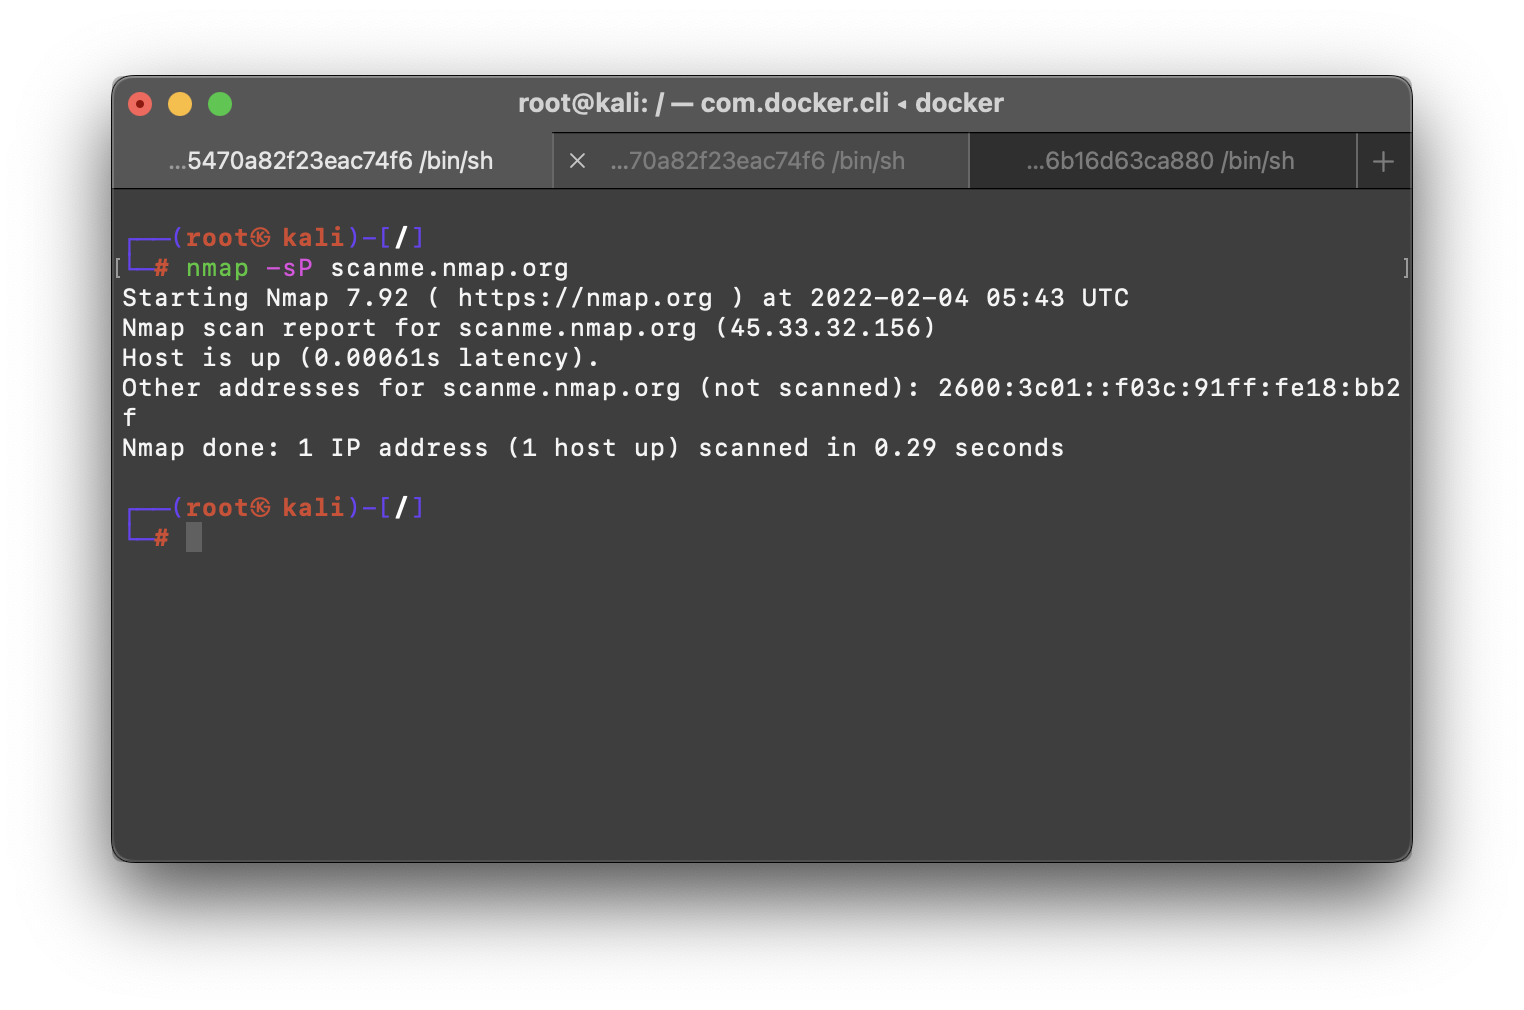
\includegraphics[width=0.6\textwidth]{figure07.png}\vspace{-1em}
    \caption{Command line for nmap of scanme.nmap.org.}
    \label{fig:nmap03}
\end{figure}

\begin{figure}[!ht]
    \centering
    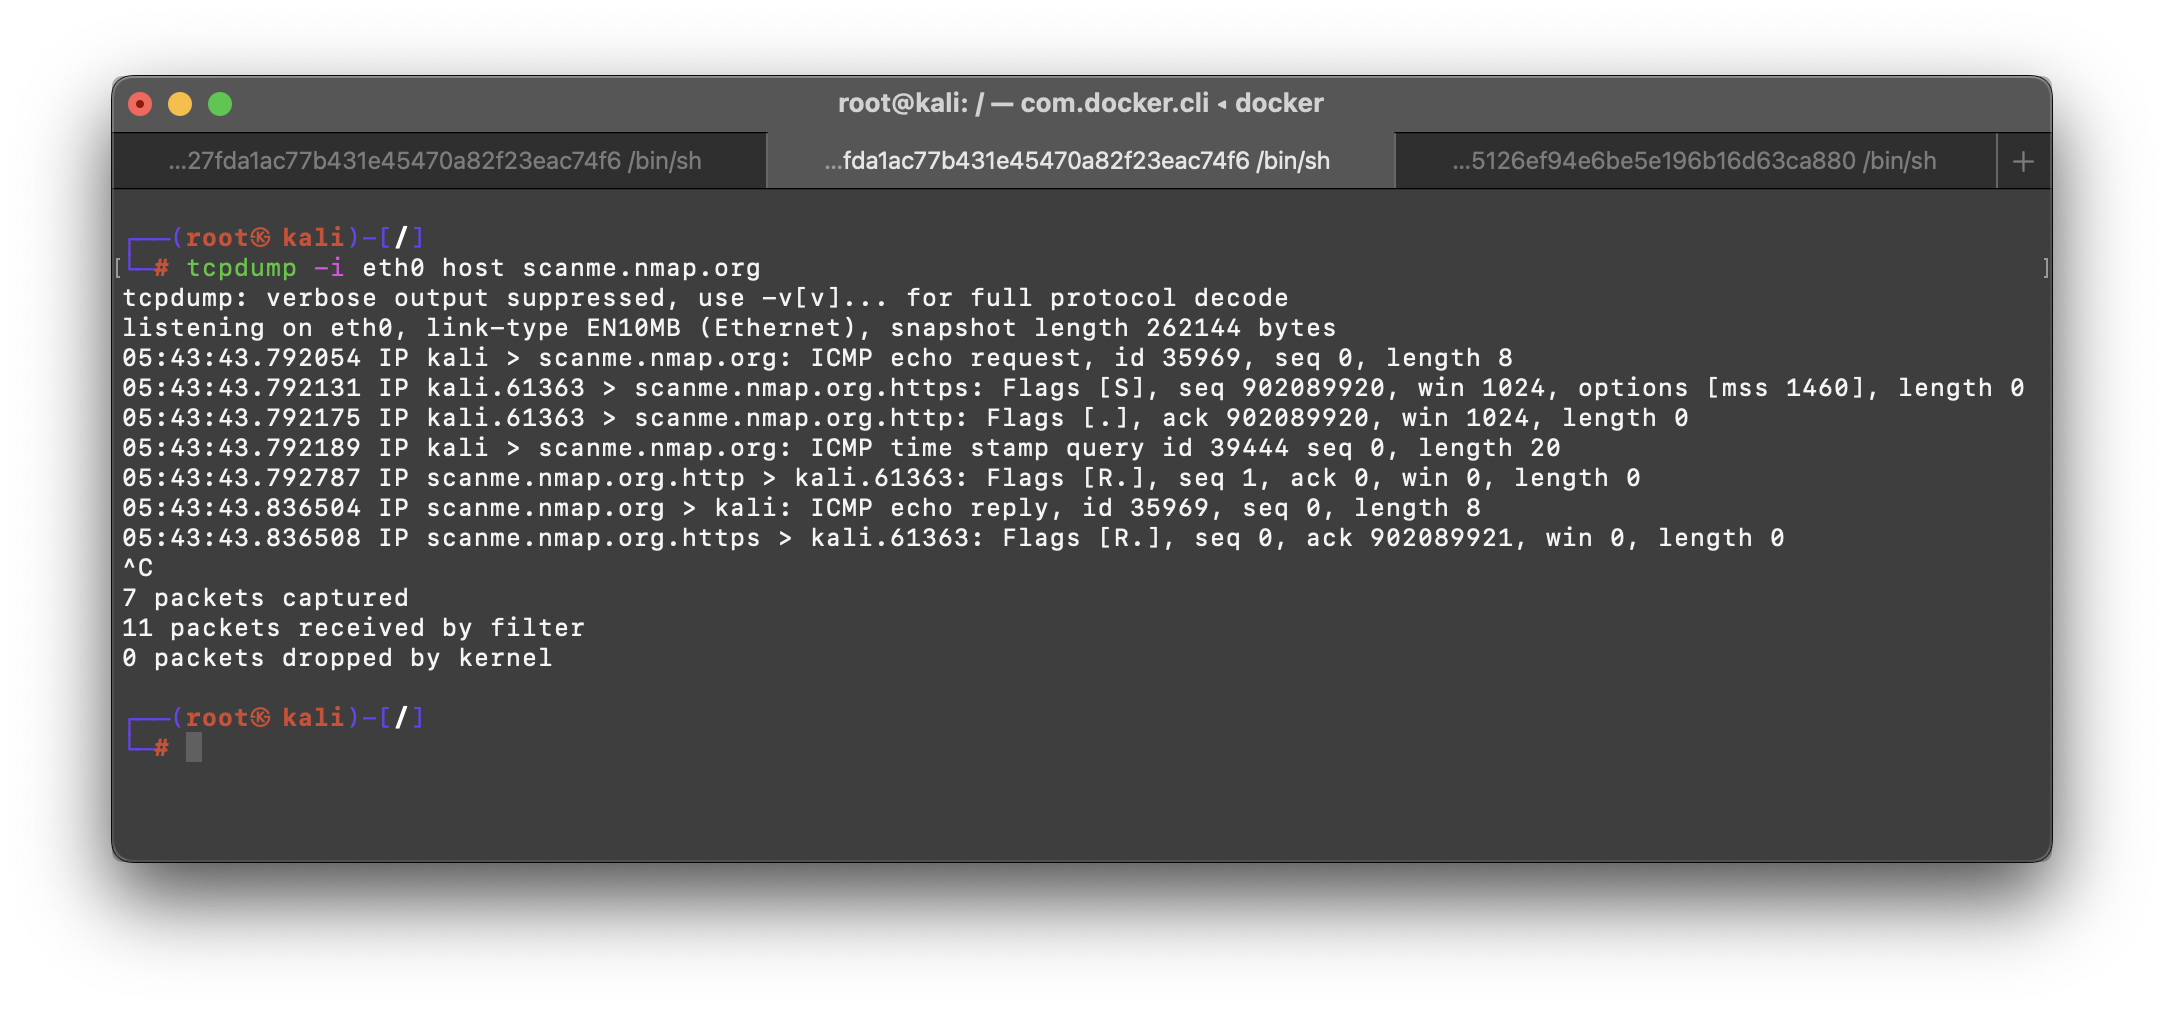
\includegraphics[width=0.8\textwidth]{figure08.png}\vspace{-1em}
    \caption{Command line for tcpdump of scanme.nmap.org.}
    \label{fig:nmap04}
\end{figure}

The third submodule was to run nmap using flags, specifically the stealth, ACK, and a mystery probe, the outputs of which are shown below. These scans show the Metasploitable container with many open ports that can be potentially exploited. This is exactly the point of this module. We see that by comparison, Kali Linux has zero open ports out of the 1000 scanned.

\begin{tcolorbox}[colback=CrispBlue!5!white,colframe=CrispBlue!75!black,title=Output of \texttt{nmap -oN stealth.txt -sS 172.17.0.*}]\setstretch{1.25}\footnotesize
\begin{verbatim}
# Nmap 7.92 scan initiated Fri Feb  4 05:50:57 2022 as: nmap -oN stealth.txt -sS 172.17.0.*
Nmap scan report for 172.17.0.1
Host is up (0.000013s latency).
Not shown: 999 closed tcp ports (reset)
PORT    STATE SERVICE
111/tcp open  rpcbind
MAC Address: 02:42:98:88:21:C2 (Unknown)

Nmap scan report for 172.17.0.2
Host is up (0.000019s latency).
Not shown: 983 closed tcp ports (reset)
PORT     STATE SERVICE
21/tcp   open  ftp
22/tcp   open  ssh
23/tcp   open  telnet
25/tcp   open  smtp
111/tcp  open  rpcbind
139/tcp  open  netbios-ssn
445/tcp  open  microsoft-ds
512/tcp  open  exec
513/tcp  open  login
514/tcp  open  shell
1099/tcp open  rmiregistry
1524/tcp open  ingreslock
2121/tcp open  ccproxy-ftp
3306/tcp open  mysql
5432/tcp open  postgresql
6667/tcp open  irc
8180/tcp open  unknown
MAC Address: 02:42:AC:11:00:02 (Unknown)

Nmap scan report for kali (172.17.0.3)
Host is up (0.0000040s latency).
All 1000 scanned ports on kali (172.17.0.3) are in ignored states.
Not shown: 1000 closed tcp ports (reset)

# Nmap done at Fri Feb  4 05:50:59 2022 -- 256 IP addresses (3 hosts up) scanned in 2.21
 seconds
\end{verbatim}
\end{tcolorbox}

\begin{tcolorbox}[colback=CrispBlue!5!white,colframe=CrispBlue!75!black,title=Output of \texttt{nmap -oN ack.txt -sA 172.17.0.*}]\setstretch{1.25}\footnotesize
\begin{verbatim}
# Nmap 7.92 scan initiated Fri Feb  4 06:03:59 2022 as: nmap -oN ack.txt -sA 172.17.0.*
Nmap scan report for 172.17.0.1
Host is up (0.0000070s latency).
All 1000 scanned ports on 172.17.0.1 are in ignored states.
Not shown: 1000 unfiltered tcp ports (reset)
MAC Address: 02:42:98:88:21:C2 (Unknown)

Nmap scan report for 172.17.0.2
Host is up (0.0000090s latency).
All 1000 scanned ports on 172.17.0.2 are in ignored states.
Not shown: 1000 unfiltered tcp ports (reset)
MAC Address: 02:42:AC:11:00:02 (Unknown)

Nmap scan report for kali (172.17.0.3)
Host is up (0.0000040s latency).
All 1000 scanned ports on kali (172.17.0.3) are in ignored states.
Not shown: 1000 unfiltered tcp ports (reset)

# Nmap done at Fri Feb  4 06:04:01 2022 -- 256 IP addresses (3 hosts up) scanned in 2.10
 seconds
\end{verbatim}
\end{tcolorbox}

\begin{tcolorbox}[colback=CrispBlue!5!white,colframe=CrispBlue!75!black,title=Output of \texttt{nmap -oN mystery.txt -Pn -sS 172.17.0.*}]\setstretch{1.25}\footnotesize
\begin{verbatim}
# Nmap 7.92 scan initiated Fri Feb  4 06:08:40 2022 as: nmap -oN mystery.txt -Pn -sS
 172.17.0.*
Nmap scan report for 172.17.0.1
Host is up (0.0000080s latency).
Not shown: 999 closed tcp ports (reset)
PORT    STATE SERVICE
111/tcp open  rpcbind
MAC Address: 02:42:98:88:21:C2 (Unknown)

Nmap scan report for 172.17.0.2
Host is up (0.000010s latency).
Not shown: 983 closed tcp ports (reset)
PORT     STATE SERVICE
21/tcp   open  ftp
22/tcp   open  ssh
23/tcp   open  telnet
25/tcp   open  smtp
111/tcp  open  rpcbind
139/tcp  open  netbios-ssn
445/tcp  open  microsoft-ds
512/tcp  open  exec
513/tcp  open  login
514/tcp  open  shell
1099/tcp open  rmiregistry
1524/tcp open  ingreslock
2121/tcp open  ccproxy-ftp
3306/tcp open  mysql
5432/tcp open  postgresql
6667/tcp open  irc
8180/tcp open  unknown
MAC Address: 02:42:AC:11:00:02 (Unknown)

Nmap scan report for kali (172.17.0.3)
Host is up (0.0000040s latency).
All 1000 scanned ports on kali (172.17.0.3) are in ignored states.
Not shown: 1000 closed tcp ports (reset)

# Nmap done at Fri Feb  4 06:08:42 2022 -- 256 IP addresses (3 hosts up) scanned in 2.20
 seconds
\end{verbatim}
\end{tcolorbox}

The fourth submodule was to use built-in flags for \textit{operating systems}, \textit{versions}, and \textit{all} to test scanme.nmap.org. The outputs are shown below, respectively.

\begin{tcolorbox}[colback=CrispBlue!5!white,colframe=CrispBlue!75!black,title=Output of \texttt{nmap -oN scanme-O.txt -O scanme.nmap.org}]\setstretch{1.25}\footnotesize
\begin{verbatim}
# Nmap 7.92 scan initiated Fri Feb  4 06:17:56 2022 as: nmap -oN scanme-O.txt -O
 scanme.nmap.org
Nmap scan report for scanme.nmap.org (45.33.32.156)
Host is up (0.029s latency).
Other addresses for scanme.nmap.org (not scanned): 2600:3c01::f03c:91ff:fe18:bb2f
Not shown: 994 closed tcp ports (reset)
PORT      STATE    SERVICE
22/tcp    open     ssh
25/tcp    filtered smtp
80/tcp    open     http
5431/tcp  filtered park-agent
9929/tcp  open     nping-echo
31337/tcp open     Elite
OS fingerprint not ideal because: Host distance (10 network hops) is greater than five
No OS matches for host
Network Distance: 10 hops

OS detection performed. Please report any incorrect results at https://nmap.org/submit/ .
# Nmap done at Fri Feb  4 06:18:02 2022 -- 1 IP address (1 host up) scanned in 5.77 seconds
\end{verbatim}
\end{tcolorbox}

\begin{tcolorbox}[colback=CrispBlue!5!white,colframe=CrispBlue!75!black,title=Output of \texttt{nmap -oN scanme-sV.txt -sV scanme.nmap.org}]\setstretch{1.25}\footnotesize
\begin{verbatim}
# Nmap 7.92 scan initiated Fri Feb  4 06:20:27 2022 as: nmap -oN scanme-sV.txt -sV
 scanme.nmap.org
Nmap scan report for scanme.nmap.org (45.33.32.156)
Host is up (0.042s latency).
Other addresses for scanme.nmap.org (not scanned): 2600:3c01::f03c:91ff:fe18:bb2f
Not shown: 994 closed tcp ports (reset)
PORT      STATE    SERVICE    VERSION
22/tcp    open     ssh        OpenSSH 6.6.1p1 Ubuntu 2ubuntu2.13 (Ubuntu Linux; protocol
 2.0)
25/tcp    filtered smtp
80/tcp    open     http       Apache httpd 2.4.7 ((Ubuntu))
5431/tcp  filtered park-agent
9929/tcp  open     nping-echo Nping echo
31337/tcp open     tcpwrapped
Service Info: OS: Linux; CPE: cpe:/o:linux:linux_kernel

Service detection performed. Please report any incorrect results at https://nmap.org/
 submit/ .
# Nmap done at Fri Feb  4 06:20:35 2022 -- 1 IP address (1 host up) scanned in 8.67 seconds
\end{verbatim}
\end{tcolorbox}

\begin{tcolorbox}[colback=CrispBlue!5!white,colframe=CrispBlue!75!black,title=Output of \texttt{nmap -oN scanme-A.txt -A scanme.nmap.org}]\setstretch{1.25}\footnotesize
\begin{verbatim}
# Nmap 7.92 scan initiated Fri Feb  4 06:21:56 2022 as: nmap -oN scanme-A.txt -A
 scanme.nmap.org
Nmap scan report for scanme.nmap.org (45.33.32.156)
Host is up (0.0089s latency).
Other addresses for scanme.nmap.org (not scanned): 2600:3c01::f03c:91ff:fe18:bb2f
Not shown: 994 closed tcp ports (reset)
PORT      STATE    SERVICE    VERSION
22/tcp    open     ssh        OpenSSH 6.6.1p1 Ubuntu 2ubuntu2.13 (Ubuntu Linux; protocol
 2.0)
| ssh-hostkey: 
|   1024 ac:00:a0:1a:82:ff:cc:55:99:dc:67:2b:34:97:6b:75 (DSA)
|   2048 20:3d:2d:44:62:2a:b0:5a:9d:b5:b3:05:14:c2:a6:b2 (RSA)
|   256 96:02:bb:5e:57:54:1c:4e:45:2f:56:4c:4a:24:b2:57 (ECDSA)
|_  256 33:fa:91:0f:e0:e1:7b:1f:6d:05:a2:b0:f1:54:41:56 (ED25519)
25/tcp    filtered smtp
80/tcp    open     http       Apache httpd 2.4.7 ((Ubuntu))
|_http-title: Go ahead and ScanMe!
|_http-favicon: Nmap Project
|_http-server-header: Apache/2.4.7 (Ubuntu)
5431/tcp  filtered park-agent
9929/tcp  open     nping-echo Nping echo
31337/tcp open     tcpwrapped
OS fingerprint not ideal because: Host distance (10 network hops) is greater than five
No OS matches for host
Network Distance: 2 hops
Service Info: OS: Linux; CPE: cpe:/o:linux:linux_kernel

TRACEROUTE (using port 80/tcp)
HOP RTT     ADDRESS
1   0.03 ms 172.17.0.1
2   0.24 ms scanme.nmap.org (45.33.32.156)

OS and Service detection performed. Please report any incorrect results at
 https://nmap.org/submit/ .
# Nmap done at Fri Feb  4 06:22:13 2022 -- 1 IP address (1 host up) scanned in 17.59
 seconds
\end{verbatim}
\end{tcolorbox}

The final submodule of Module 3 was to run built-in scripts that would emulate a few of the flags that we tested in the previous section. We found that the scripts (see Figures~\ref{fig:nmap05} and~\ref{fig:nmap06}) are not always as thorough and in-depth as the flags themselves.

\begin{figure}[!ht]
    \centering
    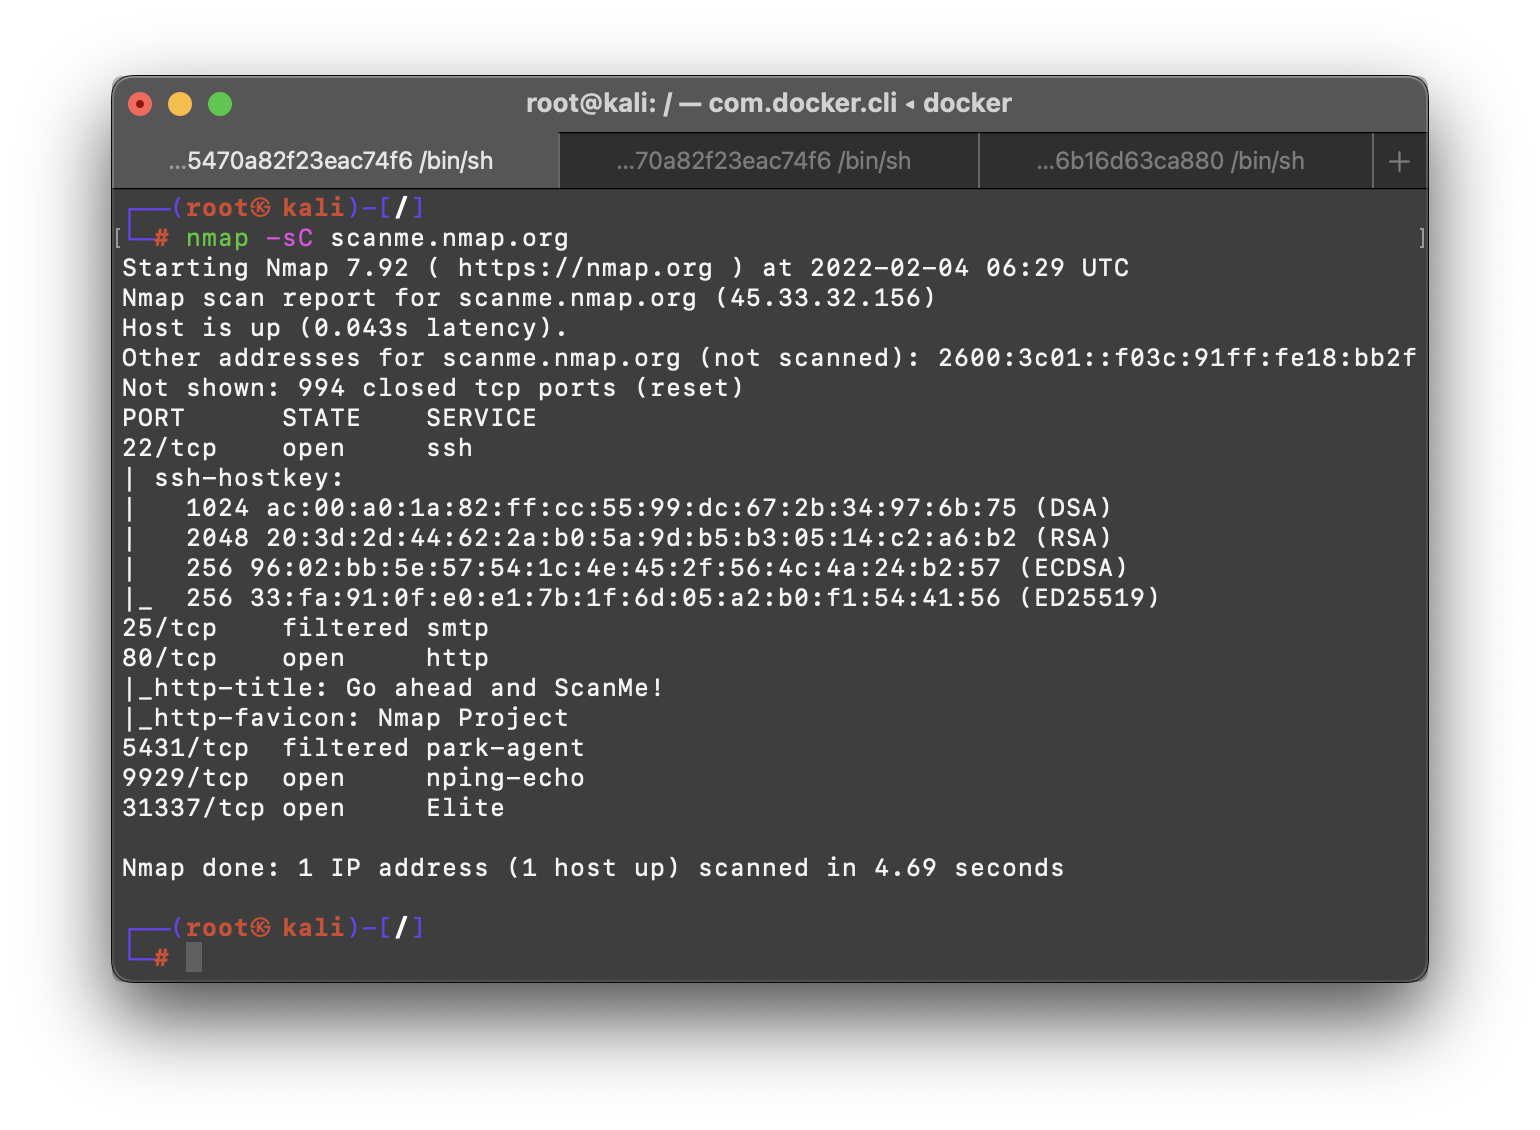
\includegraphics[width=0.8\textwidth]{figure09.png}\vspace{-1em}
    \caption{Command line for nmap with flags of scanme.nmap.org.}
    \label{fig:nmap05}
\end{figure}

\begin{figure}[!ht]
    \centering
    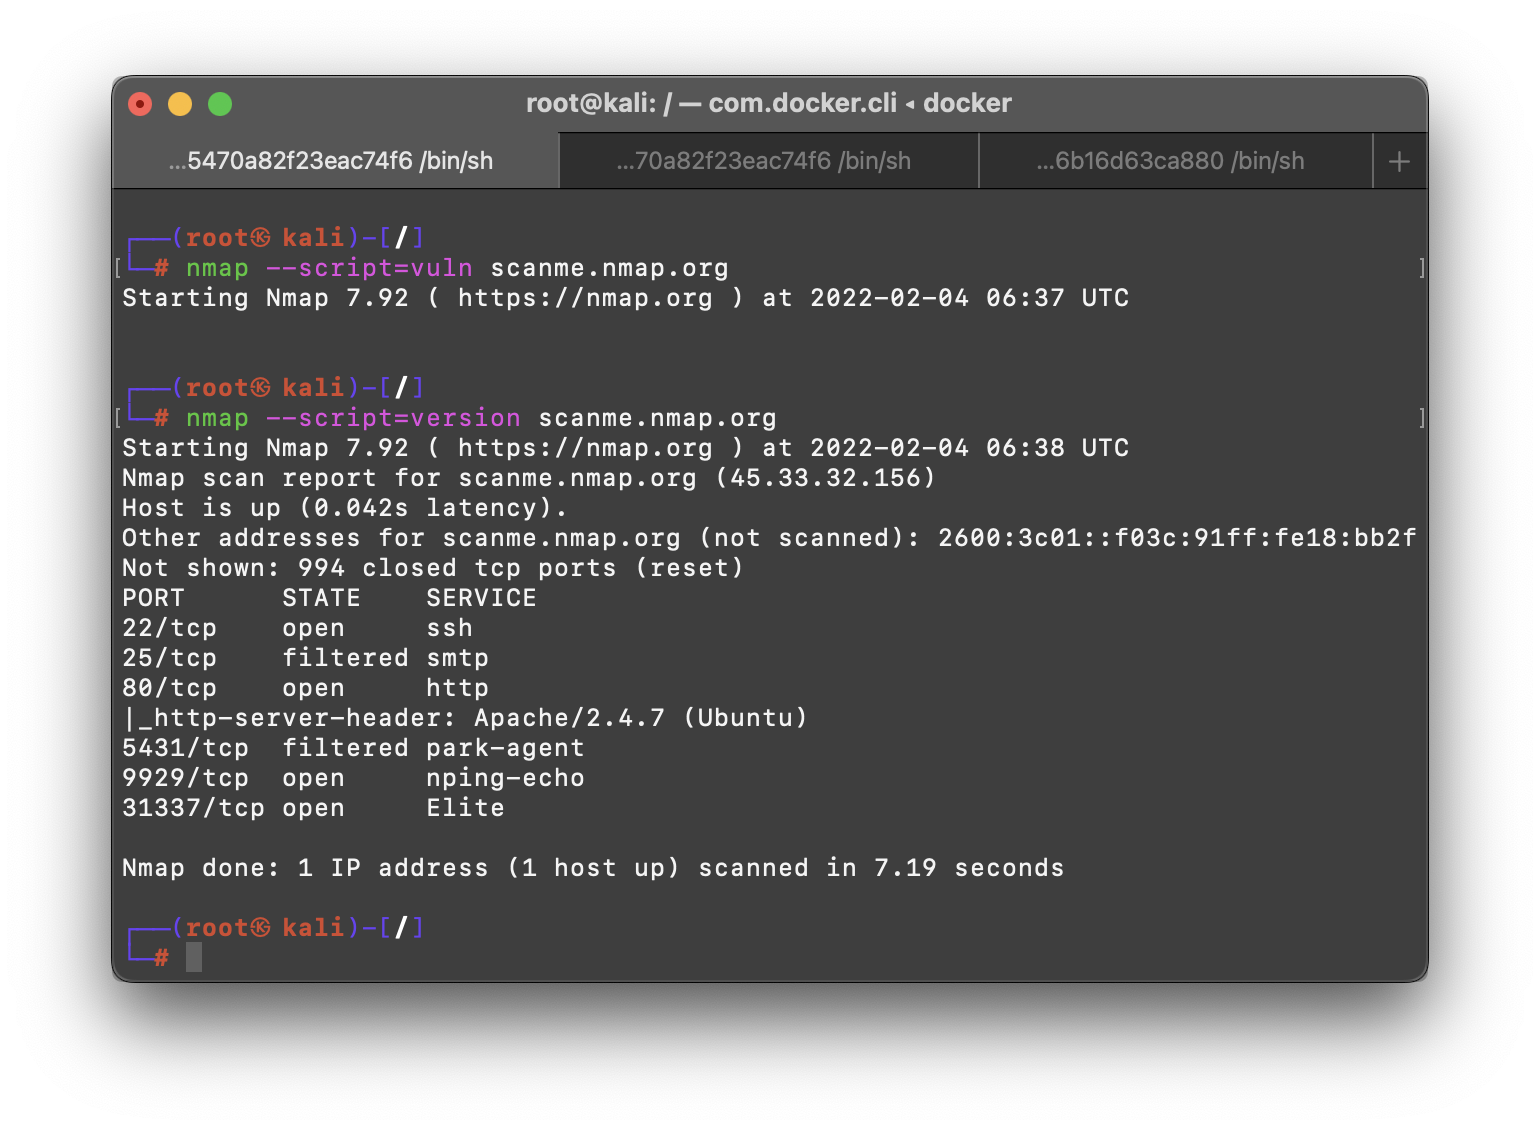
\includegraphics[width=0.8\textwidth]{figure10.png}\vspace{-1em}
    \caption{Command line for nmap with scripts of scanme.nmap.org.}
    \label{fig:nmap06}
\end{figure}


\end{document}